 \documentclass[a4paper,12pt, oneside]{book}

%  Русский язык
\usepackage{cmap}					% Улучшенный поиск русских слов
\usepackage[T2A]{fontenc}			% кодировка
\usepackage[utf8]{inputenc}			% кодировка исходного текста
\usepackage[english,russian]{babel}	% локализация и переносы
\usepackage{pscyr}					% нормальные шрифты

% Колонтитулы
\usepackage{fancybox,fancyhdr}
\usepackage{lastpage}
\fancyhf{}
\fancypagestyle{all}
{
	\fancyhead{}
	\fancyhead[C]{\vspace{-1mm}Контрольная работа 12 Вариант Попов Юрий СКБ-171}
	\fancyfoot{}
	\fancyfoot[C]{\hfill  \thepage  \hfill}
}

% Картинки и графики
\usepackage{wrapfig}
\usepackage{pgfplots}
\pgfplotsset{compat=1.9}
\graphicspath{{fotos/}}


% Ссылки
\usepackage{xcolor}
\usepackage{color,colortbl} % раскраска таблиц
\usepackage[unicode, pdftex]{hyperref}
\definecolor{linkcolor}{HTML}{000000} 	% цвет ссылок
\definecolor{urlcolor}{HTML}{8B000F}	% цвет гиперссылок
\hypersetup{urlcolor=urlcolor, linkcolor=linkcolor, colorlinks=true}

% Размеры
\setlength{\paperwidth}{210mm}
\setlength{\paperheight}{297mm}
\setlength{\textheight}{225mm} 			% высота без колонтитулов
\setlength{\textwidth}{170mm}			% ширина текста
\oddsidemargin=0pt
\setlength{\headheight}{2mm}			% высота колонтитула
\setlength{\headsep}{5mm} 	% от блока текста до верхнего колонтитула
\setlength{\footskip}{10mm}  % от блока текста до нижнего колонтитула

% Математика
\usepackage{amsmath,amsfonts,amssymb,amsthm,mathtools,mathtext} 
\usepackage{latexsym,array,epsfig,wasysym}
\usepackage[all]{xy}
\let\int\varint
\def\Int{\int\limits}
\def\IInt{\iint\limits}
\def\IIInt{\iiint\limits}
\DeclarePairedDelimiter\floor{\lfloor}{\rfloor}


% Оглавление 
\usepackage{setspace}

\usepackage{tocloft} %регулировка расположения TableOfContent (Оглавления) на странице

%\setcounter{tocdepth}{1} % отменяет вывод в оглавление subsection and subsubsection
%\setcounter{secnumdepth}{1} %отменяет номерацию секций в тексте и оглавлении.
\usepackage{tocloft} %регулировка расположения TableOfContent (Оглавления) на странице

\renewcommand{\cfttoctitlefont}{\hspace{0.38\textwidth} \bfseries\MakeUppercase} %уменьшаем размер шрифта и ровняем по центру

% % Межстрочные отступы в Оглавлении:
\setlength{\cftbeforetoctitleskip}{5mm} %отступ Оглавления от верхнего поля страницы.
\setlength{\cftbeforechapskip}{14mm} %отступ между главами
\setlength{\cftbeforesecskip}{5mm} %отступ между секциями \section{title}

% % Отступы от левого поля:
\setlength{\cftchapindent}{1mm} %отступ между левым полем и \chapter{}
\setlength{\cftsecindent}{13mm} %отступ между левым полем и \section{title}

% % Отточия в Оглавлении
\renewcommand\cftchapdotsep{\cftdot} %добавляет отточия после \chapter{title}
%\renewcommand{\cftchapleader}{\cftdotfill{\cftchapdotsep}} %делает отточия после \chapter{title} тонкими, (по умолчанию жирные).
\renewcommand\cftsecdotsep{\cftdot} %делает отточия после \section{title} частыми.

% % Интервалы между абзацами, главами и так далее:
\usepackage{titlesec}

\titleformat{\chapter}[display]
{\filcenter}
{\MakeUppercase{\chaptertitlename} \thechapter}
{2pt}
{\bfseries}{}

\titleformat{\section}
{\normalsize\bfseries}
{\thesection}
{1em}{}

\titleformat{\subsection}
{\normalsize\bfseries}
{\thesubsection}
{1em}{}

% Настройка вертикальных и горизонтальных отступов
\titlespacing*{\chapter}{10pt}{-5pt}{8pt}
\titlespacing*{\section}{\parindent}{*4}{*4}
\titlespacing*{\subsection}{\parindent}{*4}{*4}


\begin{document} % начало документа	
	\pagestyle{plain}
	
	\begin{titlepage}	
		\begin{center}
			{\Huge \textbf{Математическая статистика}}
			\vspace{30mm}
			
			{\Huge Домашняя работа № 3 \\}
			\vspace{30mm}
			
			{\huge Оценки}
			\vspace{30mm}
			
			{\Large Попов Юрий, СКБ-172}
		\end{center}
	\end{titlepage}
	
	
	
\begin{spacing}{0.99}          
	\tableofcontents %Оглавление             
\end{spacing}

\newpage
\begin{center}
	{\Huge{\bf{Предисловие}}}
\end{center}



%-------------------------------------Предисловие

Все графики, которые в дальнейшем будут вставлены в эту работу, были сконструированы с помощью различных библиотек, основные которые - это matplotlib  и numpy в Jupyter Notebook\\

К работе приложены 2 основных файла: "Geom\_Dz\_3.ipynb" и "Expon\_Dz\_3.ipynb" , в которых указаны расчеты  соотвественно геометрического и  экспоненциального распределения\\

Все фотографии, использованные в работе лежат в папке {\it fotos}\\

Когда я начинал третье домашнее задание, обновленного файла с домашней работы еще не было( или я не знал о его существовании), поэтому номер 3.2 сделан из старого файла\\


Большая часть определений, которые представлены в этой работы взять с лекций нашего курса. 
\vspace{5mm}

Также некоторые определения взяты из источника   Г.И. Ивченко, Ю.И. Медведев \\
"Ведение в математическую статистику"

%-------------------------------------Предисловие

\setcounter{secnumdepth}{-1} % убираем нумерацию 



\large\textit{\chapter{Задание 3.1 Нахождение выборочного среднего и выборочной дисперсии}}
\vspace{5mm}


\vspace{5mm}
\large{\textbf{Выборочные моменты}}
\vspace{5mm}

Наиболее важными характеристиками случайной величины $\xi$ являются ее моменты $\alpha_k = E\xi^k$, а также центральные моменты $\mu_k = E(\xi - \alpha_1)^k$( когда они существуют). Их статическими аналогами, вычисляемыми по соответствующей выборке $X = (X_1, \ldots, X_n)$, являются {\it выборочные моменты} соответственно {\it обычные}
$$
\hat{\alpha}_k = \frac{1}{n} \sum\limits_{i = 1}^n X_i^k
$$ 
и центральные 
$$
\hat{\mu}_k = \frac{1}{n} \sum\limits_{i = 1}^n (X_i - \hat{\alpha}_1)^k
$$

Особенно важны моменты первого и второго порядков.

При $k = 1$ величину $\hat{\alpha}_1$ называют {\it выборочным средним} и обозначают стандартным символом $\bar{X}$:
$$
\bar{X} = \hat{\alpha}_1 = \frac{1}{n} \sum\limits_{i = 1}^n X_i
$$

При $k = 2$ величину $\hat{\mu}_2$ называют {\it выборочной дисперсией} и  также обозначают стандартным символом $S^2 = S^2(X)$:
$$
S^2 = \hat{\mu}_2 = \frac{1}{n} \sum\limits_{i = 1}^n  (X_i - \bar{X})^2
$$

\vspace{5mm}
\phantomsection
\textbf{\section{\large{3.1.1 Геометрическое распределение}}}
\vspace{5mm}

Для каждой выборки из домашнего задания 2 посчитаем выборочное среднее и выборочную дисперсию. Для наглядности выведем вариационный ряд  для объема 5 и 10 и посчитанные оба параметра.

\begin{figure}[h!]
	\begin{center}
		\begin{minipage}[h]{0.47\linewidth}
			\center{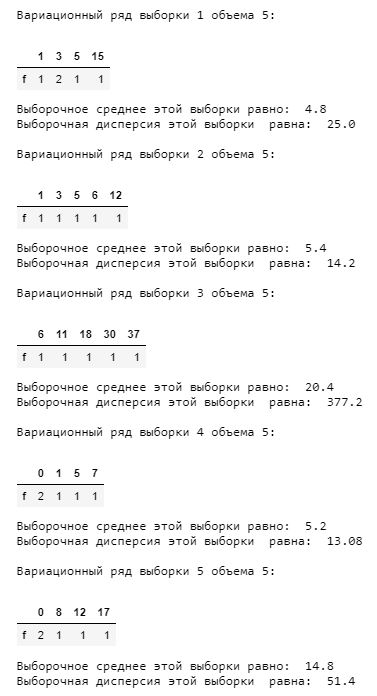
\includegraphics[width=1\linewidth]{fotos/geom_3,1_5.jpg}} n = 5 \\
		\end{minipage}
		\hfill		
		\begin{minipage}[h]{0.47\linewidth}
 			\center{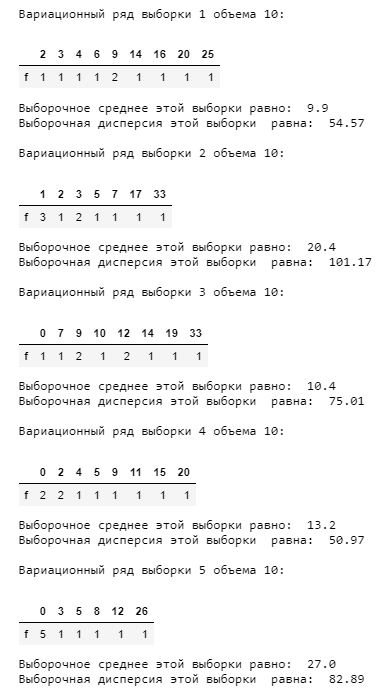
\includegraphics[width=1\linewidth]{fotos/geom_3,1_10.jpg}} n = 10 \\
		\end{minipage}
	\end{center}
\end{figure}

\begin{figure}[h!]
	\begin{center}
		\begin{minipage}[h]{0.47\linewidth}
			\center{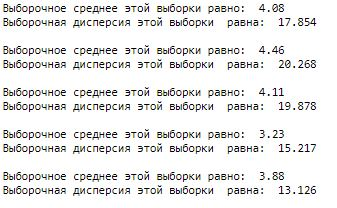
\includegraphics[width=1\linewidth]{fotos/geom_3,1_100.jpg}} n = 100 \\
			\vspace{15mm}
		\end{minipage}
		\hfill
		\begin{minipage}[h]{0.47\linewidth}
			\center{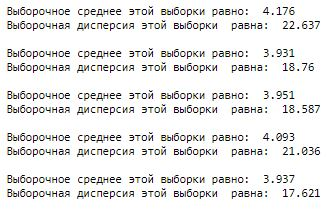
\includegraphics[width=1\linewidth]{fotos/geom_3,1_1000.jpg}} n = 1000 \\
			\vspace{5mm}
		\end{minipage}
		\hfill
		\begin{minipage}[h]{0.47\linewidth}
			\center{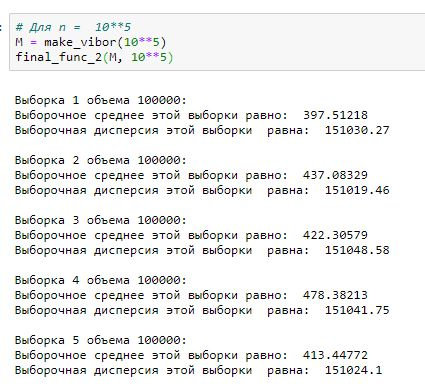
\includegraphics[width=1\linewidth]{fotos/geom_3,1_103.jpg}} n = 100000 \\
			\vspace{5mm}
		\end{minipage}	
	\end{center}
\end{figure}

\newpage
$$
\\
\\
\\
\\
\\
\\
$$



\newpage
\textbf{Свойства выборочного среднего}


\vspace{5mm}
{\sf$\bullet$ Выборочное среднее — несмещённая оценка теоретического среднего:}
\vspace{5mm}

\vspace{5mm}
{\sf$\bullet$ Выборочное среднее — сильно состоятельная оценка теоретического среднего:}
\vspace{5mm}

\vspace{5mm}
{\sf$\bullet$ Выборочное среднее — асимптотически нормальная оценка.}
\vspace{5mm}

\vspace{5mm}
{\sf$\bullet$ Выборочное среднее из нормальной выборки — эффективная оценка её среднего.}
\vspace{5mm}


\vspace{5mm}
\phantomsection
\section{3.1.2 Экспоненциальное распределение}
\vspace{5mm}


Для каждой выборки из домашнего задания 2 посчитаем выборочное среднее и выборочную дисперсию. Для наглядности выведем вариационный ряд  для объема 5 и 10 и посчитанные оба параметра.

\begin{figure}[h!]
	\begin{center}
		\begin{minipage}[h]{0.47\linewidth}
			\center{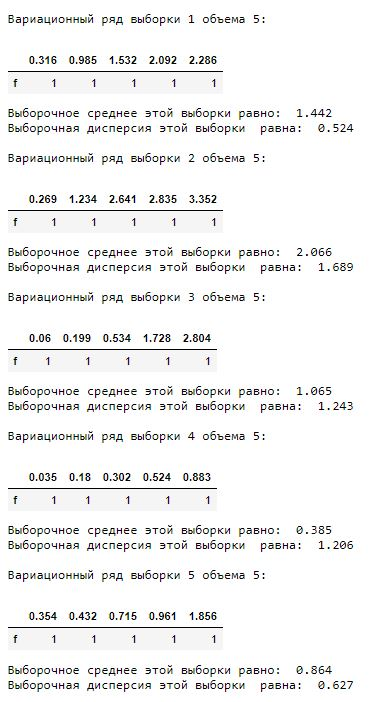
\includegraphics[width=1\linewidth]{fotos/expon_3,1_5.jpg}} n = 5 \\
			\vspace{15mm}
		\end{minipage}
		\hfill		
		\begin{minipage}[h]{0.47\linewidth}
			\center{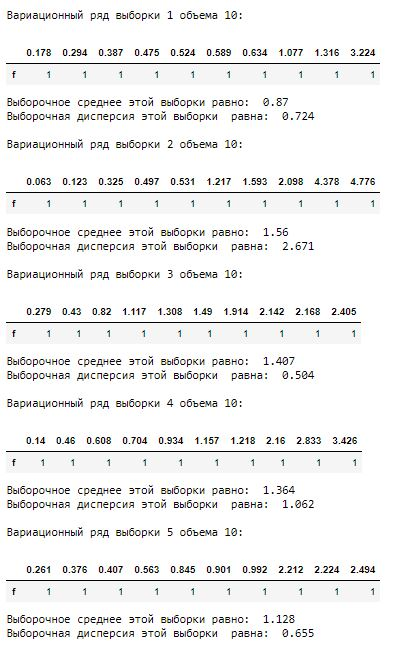
\includegraphics[width=1\linewidth]{fotos/expon_3,1_10.jpg}} n = 10 \\
			\vspace{15mm}
		\end{minipage}	
	\end{center}
\end{figure}

\begin{figure}[h!]
	\begin{center}
		\begin{minipage}[h]{0.47\linewidth}
			\center{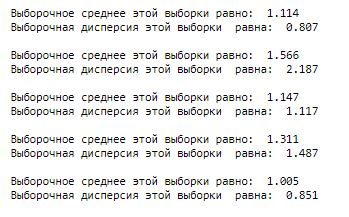
\includegraphics[width=1\linewidth]{fotos/expon_3,1_100.jpg}} n = 100 \\
			\vspace{15mm}
		\end{minipage}
		\hfill
		\begin{minipage}[h]{0.47\linewidth}
			\center{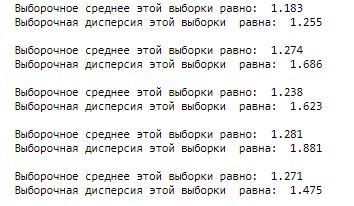
\includegraphics[width=1\linewidth]{fotos/expon_3,1_1000.jpg}} n = 1000 \\
			\vspace{5mm}
		\end{minipage}
		\hfill
		\begin{minipage}[h]{0.47\linewidth}
			\center{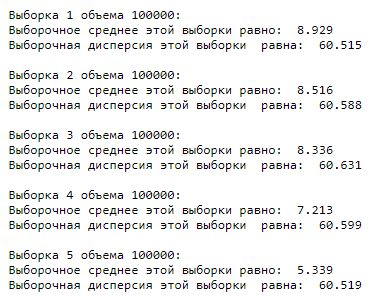
\includegraphics[width=1\linewidth]{fotos/expon_3,1_103.jpg}} n = 100000 \\
			\vspace{5mm}
		\end{minipage}	
	\end{center}
\end{figure}


\phantomsection
\large{ \it \chapter{ Задание 3.2 Построение доверительного интервала для выборочного среднего и выборочной дисперсии}}
\vspace{5mm}



\vspace{5mm}
\phantomsection
\textbf{\section{\large{3.2.1 Геометрическое распределение}}}
\vspace{5mm}

Для всех выборок построим доверительные интервалы.

\begin{figure}[h!]
	\begin{center}
		\begin{minipage}[h]{0.47\linewidth}
			\center{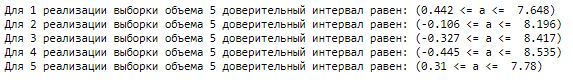
\includegraphics[width=1\linewidth]{fotos/geom_dov_interval_5.jpg}} n = 5 \\
			\vspace{15mm}
		\end{minipage}
		\hfill
		\begin{minipage}[h]{0.47\linewidth}
			\center{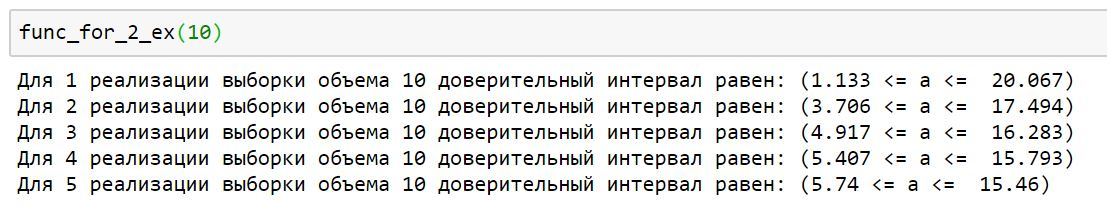
\includegraphics[width=1\linewidth]{fotos/geom_dov_interval_10.jpg}} n = 10 \\
			\vspace{15mm}
		\end{minipage}
		\hfill
		\begin{minipage}[h]{0.47\linewidth}
			\center{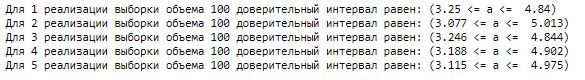
\includegraphics[width=1\linewidth]{fotos/geom_dov_interval_100.jpg}} n = 100 \\
			\vspace{15mm}
		\end{minipage}
		\hfill
		\begin{minipage}[h]{0.47\linewidth}
			\center{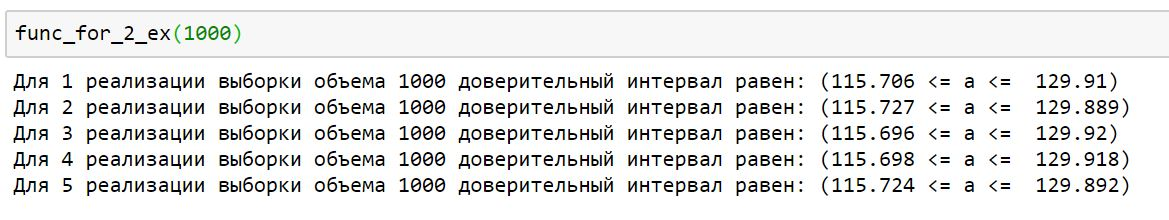
\includegraphics[width=1\linewidth]{fotos/geom_dov_interval_1000.jpg}} n = 1000  \\
			\vspace{15mm}
		\end{minipage}
		\hfill	
		\begin{minipage}[h]{0.47\linewidth}
			\center{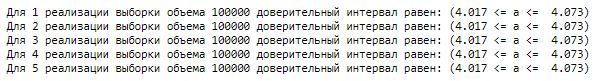
\includegraphics[width=1\linewidth]{fotos/geom_dov_interval_103.jpg}} n = 100000 \\
		\end{minipage}
	\end{center}
\end{figure}




\vspace{5mm}
\phantomsection
\textbf{\section{\large{3.2.2 Экспоненциальное распределение}}}
\vspace{5mm}

Для всех выборок построим доверительные интервалы.

\begin{figure}[h!]
	\begin{center}
		\begin{minipage}[h]{0.47\linewidth}
			\center{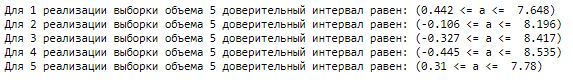
\includegraphics[width=1\linewidth]{fotos/geom_dov_interval_5.jpg}} n = 5 \\
			\vspace{15mm}
		\end{minipage}
		\hfill
		\begin{minipage}[h]{0.47\linewidth}
			\center{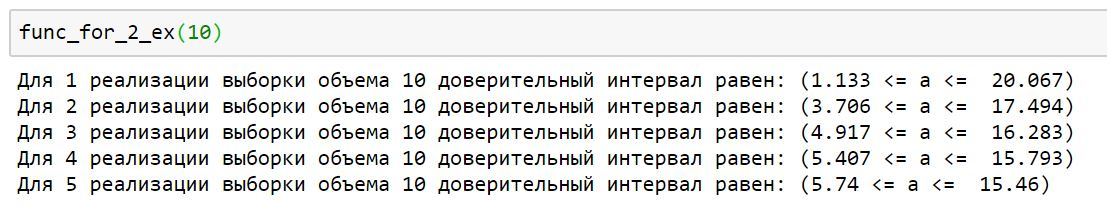
\includegraphics[width=1\linewidth]{fotos/geom_dov_interval_10.jpg}} n = 10 \\
			\vspace{15mm}
		\end{minipage}
		\hfill
		\begin{minipage}[h]{0.47\linewidth}
			\center{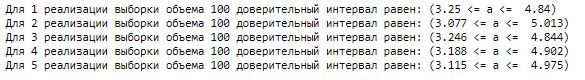
\includegraphics[width=1\linewidth]{fotos/geom_dov_interval_100.jpg}} n = 100 \\
			\vspace{15mm}
		\end{minipage}
		\hfill
		\begin{minipage}[h]{0.47\linewidth}
			\center{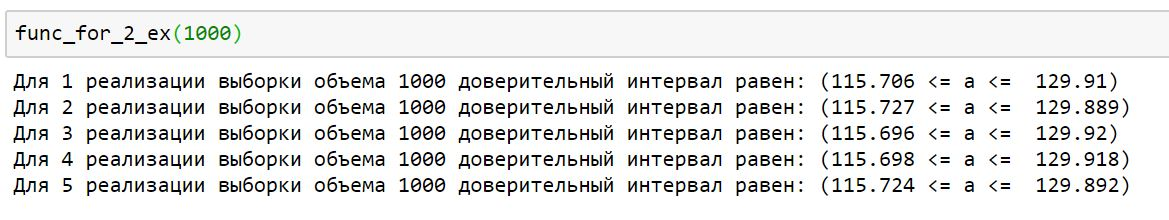
\includegraphics[width=1\linewidth]{fotos/geom_dov_interval_1000.jpg}} n = 1000  \\
			\vspace{15mm}
		\end{minipage}
		\hfill	
		\begin{minipage}[h]{0.47\linewidth}
			\center{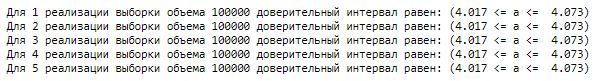
\includegraphics[width=1\linewidth]{fotos/geom_dov_interval_103.jpg}} n = 100000 \\
		\end{minipage}
	\end{center}
\end{figure}



\phantomsection
\vspace{5mm}
\large\textit{\chapter{Задание 3.3 Нахождение параметров распределений событий}}



\vspace{5mm}
\phantomsection
\textbf{\section{\large{3.3.1 Геометрическое распределение}}}
\vspace{5mm}

Найдем оценку для геометрического распределения
$$
P(X=k) = q^{k - 1} p 
$$

Найдём истинные первый и центральный второй моменты геометрического распределения:

$$
\overline{x} = M_1 = \sum_{k=1}^{\infty} p q^{k-1} k = p \sum_{k=1}^{\infty} q^{k-1} k = \dfrac{1}{p}
$$

$$
D = M_c^2 = E(x - \overline{x})^2 = \sum_{k=1}^{\infty} q^{k-1} k^2 = \dfrac{q}{p^3} = M_1 \dfrac{q}{p^2}
$$

\textbf{Метод моментов}

По методу моментов находим оценку параметра p: $ p = \dfrac{1}{x} $

Точечной оценкой параметра p является $ \dfrac{1}{\overline{x}} $

\textbf{Метод максимального правдоподобия}
$$
L(x_1, x_2, \cdots, x_n; \theta) = p^n q^{n(\theta - 1)}
$$

$$
\ln(L) = n \ln(p) + n(\theta - 1)\ln(q)
$$

$$
\dfrac{\partial \ln(L)}{\partial \theta} = n \ln q = 0
$$

Минимума или максимума нет. Т.е. метод максимального правдоподобия не работает в случае геометрического распределения

\vspace{5mm}
\phantomsection
\textbf{\section{\large{3.3.2 Экспоненциальное распределение}}}
\vspace{5mm}



\textbf{Оценка методом моментов}

Математическое ожидание равно $ Ex = \theta + \dfrac{1}{\lambda} $

Дисперсия равна $ Dx = \dfrac{1}{\lambda^2} $

$$
\bar{x} = \theta + \dfrac{1}{\lambda}
$$

Оценка: 

$$
\theta_\text{омм} = \bar x - \dfrac{1}{\lambda}
$$

Проверим, является ли данная оценка несмещенной

$$
E_\theta T = E\left( \bar X - \dfrac{1}{\lambda} \right) = E\bar{X} - \dfrac{1}{\lambda} = \theta + \dfrac{1}{\lambda} - \dfrac{1}{\lambda} = \theta
$$

Следовательно, оценка $ \theta_\text{омм} $ несмещенная оценка параметра $ \theta $

$$
D\theta_\text{омм} = D\left( \bar X - \dfrac{1}{\lambda} \right) = D(\bar{X}) + 0 =  D(\bar{X}) = \dfrac{1}{n^2} D\left( \sum_{i=1}^{n} x_i \right) = \dfrac{1}{n^2} \dfrac{1}{\lambda^2} = \dfrac{1}{n \lambda^2} \to 0 ghb n \to \infty
$$

Следовательно, $ \theta_\text{омм} $ состоятельная оценка параметра $ \theta $

\textbf{Оценка максимальным правдоподобием}

$$
\theta_\text{омм} = argsup L(x; \theta)
$$

$$
L(x;\theta) = \lambda^n e^{-\lambda \sum_{i=1}^n (x_i - \theta)}
$$

Воспользуемся тем, что экстремумы $ L(x; \theta) $ и $ \ln L(x; \theta) $ совпадают

$$
\ln L (x; \theta) = \ln \lambda^n e^{-\lambda \sum_{i=1}^n (x_i - \theta)} = n \ln \lambda - n \lambda \bar{X} + n \lambda \theta 
$$

$$
\dfrac{\partial \ln L(x; \theta)}{\partial \theta} = n \lambda > 0
$$

Чтобы максимизировать функцию правдоподобия, возьмем максимальное $ \theta $

$$
\theta_\text{омм} = X_{(1)}
$$

Проверим несмещенность оценки

$$
F_{(1)} (x) = 1 - (1 - F(x))^n = 1-(1-1+e^{- \lambda (x - \theta)})^n = 1 - \left(  \dfrac{e^{\lambda n}}{e^{\lambda \theta}} \right)^n = 1 - \dfrac{e^{\lambda \theta n}}{e^{\lambda x n}}
$$

$$
f_{(1)} (x) = F'_(1)(x) = \dfrac{e^{\lambda n} \lambda n}{e^{\lambda x n}} = \lambda n e^{-\lambda n (x- \theta)}
$$


$$
\begin{array}{rcl}
	E_\theta x_{(1)} &=&\\
	\\
	\int_{0}^{\infty} x f_{(1)} (x; \theta) dx &=&\\
	\\
	\int_{0}^{\infty} x \lambda n e^{-\lambda n (x- \theta} &=&\\
	\\
	\lambda n e^{\lambda n \theta} \left( - \dfrac{x e^{- \lambda x n}}{\lambda n} + \dfrac{1}{\lambda n} \int_{0}^{\infty} e^{-\lambda n x}dx \right) &=& \\
	\\
	  -x e^{-\lambda n (x- \theta)}\mid_0^\infty - \dfrac{\lambda n e^{\lambda n (x - \theta)}}{\lambda^2 n^2}\mid_0^\infty &=&
	  \\
	   \theta + \dfrac{1}{\lambda n}
\end{array}
$$

Таким образом, оценка максимальным правдоподобием смещена со смещением $ \frac{1}{\lambda n} $

$$
\theta = X_{(1)} - \frac{1}{\lambda n}
$$

Найдем дисперсию несмещенной оценки:

$$
D\theta_\text{омп} = D\left( X_{(1) - \frac{1}{\lambda n}}\right) = EX_{(1)}^2 - (EX_{1})^2 = \theta^2 - \dfrac{2 \theta}{\lambda n} - \dfrac{2}{\lambda^2 n^2} - \left( \theta + \dfrac{1}{\lambda n}\right)^2 = \dfrac{1}{(\lambda n)^2}
$$

$D\theta_\text{омп} \to 0  $ при $ n \to \infty \to $ оценка состоятельна

\textbf{Эффективная оценка}

х зависит от параметра $\theta \to$ модель не регулярна $ \to $ не существует эффективной оценки 


\begin{thebibliography}{99}
	\bibitem{rt1} 
	\bibitem{rt2} \href{https://towardsdatascience.com/what-is-exponential-distribution-7bdd08590e2a}{ссылка1}
	\bibitem{rt3}  \href{https://www.statisticshowto.datasciencecentral.com/exponential-distribution/}{ссылка2}
	\bibitem{rt4}  // \href{http://www.ams.jhu.edu/~dan/550.435/notes/COURSENOTES435.pdf}{ссылка3}
	\bibitem{rt5}  // \href{http://www.obzh.ru/nad/4-3.html}{ссылка4}
\end{thebibliography}

\end{document}